\chapter{Conclusion \& Future Work}\label{chap:conclusion}

\section{Conclusion}

In our preparation for dissertation we explored and presented the problem of software merges, more specifically, the difficulty in establishing an automated method to detect, identify and highlight semantic conflicts that arise.

We explored related work that can provide avenues of study and structures to guide the development of our solution. Specifically, previous work on test generation to identify semantic conflicts, the state of the art of automated test generation and the usage of Large Language Models for test generation, with specific focus on the important of appropriate prompting as well as output correction.

By establishing the three research question we established, we could investigate the viability of using LLMs in this way. From this we can say:

\begin{itemize}
\item Research Question 1: We established that ChatGPT has some capability to identify semantic conflicts. One of the obstacles found was understanding:
conflicts which did not create obvious code faults (such as parallel addition to lists) were not seen as conflicts. 

\item Research Question 2: We found that despite many small errors with the test setup and asserts, when an appropriate explanation was given, ChatGPT could generate
tests that appropriately verified the required behaviours. We also found no significant difference between human written and ChatGPT written explanations. The main obstacle
was the complexity of some subjects, particularly the real-world ones, where ChatGPT struggled to generate adequate tests.

\item Research Question 3: By investigating state of the art prompts, we observed that while they could still generate tests that adequately tested the conflict (after correction),
these came with downsides, due to the lack of focus provided by the detailed explanation: there was higher variability as it was not guaranteed the right setup would be attempted.
For example, in tests that required a User class to have the admin field set to true, nothing in the prompt indicated this and while generating many tests will increase the chances
of this field being set, more tests necessarily imply more time and work.
\end{itemize}

Forward, future work may hopefully apply this knowledge in developing a solution that can hopefully aid developer workflows by identifying and generating tests for semantic conflicts.

\section{Future Work}

During the course of our research we found many possible future avenues of research based both on our own work and existing research. Future work which explores these could improve
the quality of our prompting techniques and eventually developed a solution to automatically generate appropriate unit tests when a semantic merge conflict is detected in a commit.

Future improvements to prompting include:

\begin{itemize}
\item Improving understanding of semantic conflicts: As the LLM demonstrated an association between unintended software faults and conflicts, simple conflicts were ignored.
Possible work could focus on providing k-shot learning to improve this capability, or avoid the usage of ``conflict'' in favour of more direct or neutral terms, such as prompting
for the existence of lost or emergent behaviour.

\item Prompt automation and picking necessary information: For our purposes, prompts were manually written. To fit within token limits and to avoid confusing the LLM, informed was cropped to
the necessary: only the class were the main affected method was present was given. In the case of real-world scenarios, diffs were also cropped, as they included a lot of extraneous information.
In an automated solution, investigation needs to be done on identifying the necessary elements required for the prompt and how to automatically extract them.

\item Test generation with context: Throughout all our test generations, compilations tended to fail due to small errors, particularly with constructors, field access and method calls.
Providing context by prompting with an existing suite has shown to be a reliable solution and would also aid in following stylistically conventions a project may be using.
This could also be helpful with other issues, such as using mocking and more complex techniques when and only when it is necessary.

\item Integration with Changes-Matcher\Citet{kn:nuno}: Changes-Matcher detects semantic conflicts by comparing merges to common patterns, such as Change Method, Parallel Field and others
seen throughout our work. Integrating these, possibly with a prompt to explain the specific type of conflict present could be helpful in conflict explanation.
Furthermore, Changes-Matcher outputs a DSL which provides information on how to test the conflict (indicating which methods should be called directly and indirectly). This could possibly
also improve test generation.
\end{itemize}

\subsection{Development Plan and Tool Functioning}
todo{
Development of the solution will go through several stages. Firstly, the process which has already been in progress, is the initial evaluation of LLM's and prompt techniques. After acquiring the list of subjects to test and deciding on the LLM, we can systematize this to develop the prototype solution. From here we start developing a tool that can automatically generate a prompt, get a test from the LLM and then run it. This prototype tool can then be further augmented, by applying corrections for tests that may fail to compile. \Cref{fig:tool} details the expected functioning of the tool once completed. A final period of evaluation and observations will compare our results to previous work and reflect on possible further improvements.
}
\begin{figure}
    \centering
    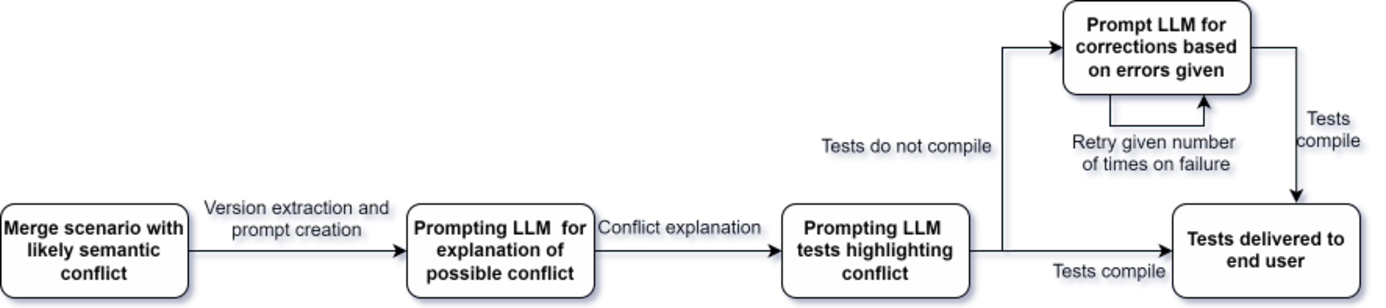
\includegraphics[width=1\linewidth]{figures/tool.pdf}
    \caption{Functioning pipeline of proposed tool.\todo{good enough? check svg better}}
    \label{fig:tool}
\end{figure}